
\section{How to Analyze Usage Data}

Thus far we have been focusing on concrete usage data collection frameworks and the specific data collected by these frameworks. When analyzing this data, or data from other collection frameworks, data analysis follows several predictable patterns, which we discuss in this section. However, we first discuss the nature of the collected data, especially whether it is anonymous, which dramatically effects how it is analyzed.

\subsection{Types of Data}

\vspace{0.1in}

\noindent
{\bf Anonymous data}, where only records of activities and anonymous facts about artifacts are recorded, may at first seem strictly inferior. Indeed there are some limitations around what can be inferred from anonymous activity streams. Yet the advantages make it a great complementary data source. First, developers are receptive to data collection for research purposes, and thus the ability to collect a large amount of information from many developers increases greatly. Second, because of this larger collection, while it may be more difficult to analyze anonymous data, any conclusions made on a larger data set collected from working developers are ultimately more believable, as they represent actual field usage. 

In this section we focus on analyzing anonymous data sources. We do so because analyzing anonymous activity streams is similar to analyzing non-anonymous data streams (i.e., they are both activity streams) and because the unlimited variation of analysis permitted by non-anonymous data affords few generalities. As we discuss analyzing usage data we start with straightforward magnitutde analysis, build to a categorization system for activity streams, and finally discuss dividing streams into sessions. 


\subsection{Usage Data Format}
Most usage data is collected as an activity stream with varying levels of supporting detail. In Figure~\ref{fig:theoretical} we present an abstraction of a typical activity stream. It includes a timestamp, followed by the activity, appended with (often anonymous) details concerning that activity. We can apply this model to the examples discussed earlier. For instance, the Mylyn Monitor's interaction event corresponds to a row in our theoretical model. It includes a timestamp (i.e., StartDate), an activity description (i.e., Kind, OriginId), and additional information (i.e., StructureHandle, StructureKind). Similarly, the CodingSpectator example includes a timestamp (i.e., stamp), an activity description (i.e., id), and a much larger set of additional information (i.e., code-snippet, selection, selection-in-code-snippet, etc.). Because these and other usage data activity streams can easily be described using our abstraction we will refer to it as we describe data analysis techniques.


%TODO: Rewrite/Adapt/Remove this paragraph now that it's been integrated

%What do they look like

%include theoretical example

%several concrete examples (codingsepctator, Sando, Eclipse study)

%Software systems often keep a record about what event was completed (or not) in the form of a log file. The information collected in the log file is often used for diagnostic purposes. If a system failure occurs, the logs for that period can be inspected to see which sequence of events were executed by the system and what were the values for the dynamic information in those events. Each log line can be traced back to a particular line of code where the method to log this information was called. Hene, we can get complete information on what events were executed. The log message store information about the branches taken by that particular instance of execution and the values for variables in the code. Due to these reasons, the information in the log file is collected as a serially ordered flat text file. In short, a log file is a collection of log lines, with each of them having information about a single event, its time of execution and the dynamic information about variable values. Note that each log line may span across multiple lines, but provides information to distinct two adjacent log lines.



\begin{figure*}[t]
 \centering
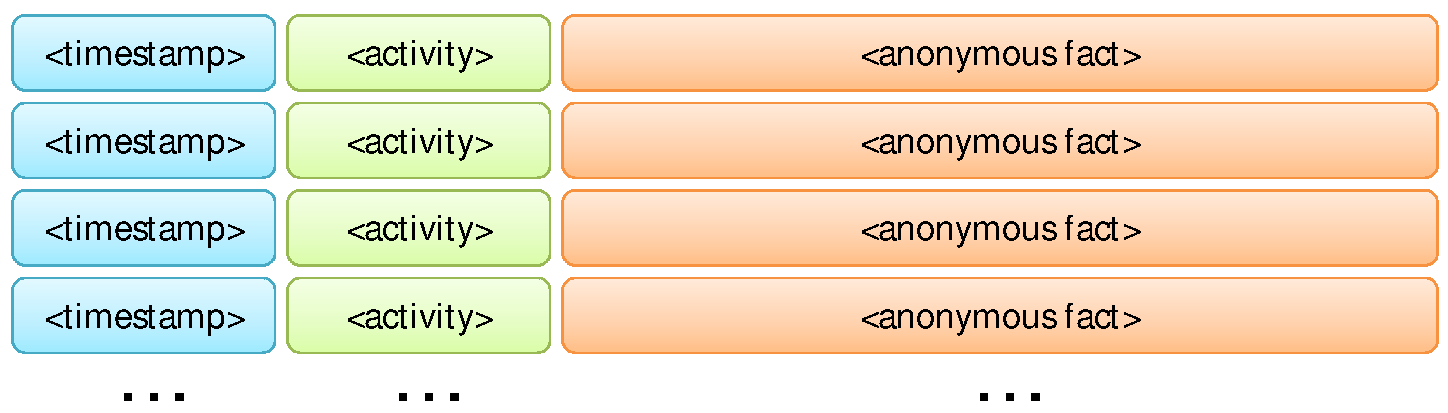
\includegraphics[width=1\columnwidth]{activityLogTheoretical.pdf}
\caption{Abstract model of developer activity streams.}
\label{fig:theoretical}
\end{figure*}



%\begin{figure*}[t]
 %\centering
%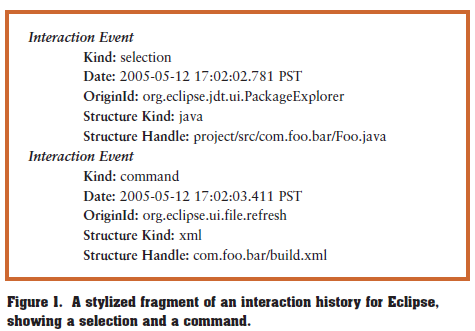
\includegraphics[width=0.5\columnwidth]{activityEvent}
%\caption{Activities as Captured in an Eclipse Usage Data Study}
%\label{fig:activity}
%\end{figure*}
%
%\begin{figure*}[t]
 %\centering
%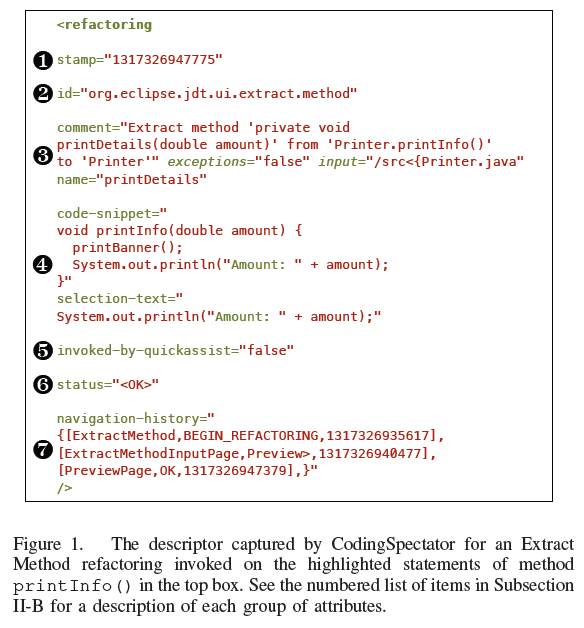
\includegraphics[width=0.5\columnwidth]{codingSpectator}
%\caption{Activities as Captured in a CodingSpectator Study of Refactoring Events}
%\label{fig:activit}
%\end{figure*}



\subsection{Magnitude Analysis}
A major advantage of anonymous usage data is the fact that it captures developers in their natural habitat, without any observational bias. Deriving conclusions from hours of developers' field work is naturally more convincing than from hour-long, in-lab user studies. One type of questions that usage data is well-suited to answer uses measurement of the magnitude of occurence of a specific event. For instance, researchers may want to know ``How often do developers invoke the pull-up refactoring'' or ``How often is the file search invoked?''. By performing a count of a specific message in the collected logs, researchers can easily calculate frequencies of specific actions that can be often sufficient to answer important research questions. However, researchers must be wary of a few common issues with magnitude analysis. First, in any sufficiently large set of user logs there is a small set of users that will use the feature/tool under analysis orders of magnitude more often than the general population, potentially skewing the data. Second, any fine-grained attempt to qualify the raw counts requires making possibly incorrect assumptions about the data. For instance, there is a temptation to report refactorings per hour, yet any fine-grained time calculation requires assumptions about how time was spent between activities, which experience has taught us are often wrong. Note that coarse-grained qualification, such as refactorings performed per day, are possible.   

%example
\begin{figure}
  \centering
  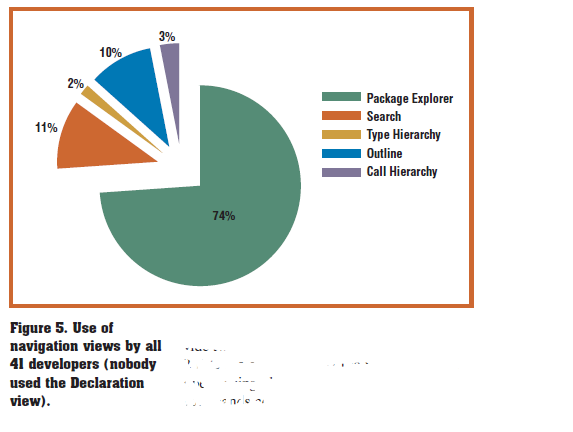
\includegraphics{AnalyzingUsageData/eclipse}
  \caption{Breakdown of Navigation-Focused View Usage in Eclipse}\label{fig:eclipse}
\end{figure}




\subsection{Categorization Analysis}
While magnitude analysis is well-suited for answering research questions about the use of a single IDE command, many research questions are related to a specific part or tool in the IDE, which usually corresponds to multiple IDE commands. For instance, the research question ``How often are refactorings performed?'' cannot be answered via magnitude analysis alone, as refactorings can be triggered through a number of different IDE commands. These commands first need to be categorized, after which magnitude analysis can be used. When focusing on a concrete sub-task, such as refactoring, it may be easy to categorize activities. In this case, all refactoring commands, such as pull-up or extract method, can be classified as refactorings. However, when focusing on more general behavior, such as editing, navigating, and searching, categorization can be difficult. It is impossible to say, for instance, from a single click in the {\tt File Explorer} window, whether that click represents a search, as the developers browses a few promising files, or a navigation, as he implicitly opens a type declaration of a variable he was just browsing. Thus, categorization without context can produce noisy data in certain cases. However, caterigorization is a powerful tool, especially when there is little ambiguity in the IDE commands that are analyzed.

To illustrate both the power and limitations of category analysis consider the following IDE data stream, and the research questions ``Do developers use code search tools?''. 

\begin{verbatim}
Collector Started
2014-02-02 13:21:22 - User submitted query to Find-in-Files
2014-02-02 13:24:36 - Find-in-Files retreived 42 results
2014-02-02 13:32:21 - User clicked on result 2
2014-02-02 13:46:56 - User submitted query to Quick Find
2014-02-02 14:07:12 - Open definition command; input=class
...
2014-02-02 14:46:52 - User submitted query to Find-in-Files
2014-02-02 14:46:56 - Find-in-Files retreived 8 results
2014-02-02 14:48:02 - Click on File Explorer
...
\end{verbatim}

For this research question, the category of log events related to code search tools should be identified and counted. Modern IDEs commonly offer several code search tools, which operate at the global or local scale, such as the {\tt Find-in-Files} and
the {\tt Quick Find} tools in the above example based on Visual Studio. Using categorization analysis we can identify three
log events related to usage of code search tools, and report various statistics aimed at answering the research question (e.g. number of code search events per day, number of code search events per user). However, the IDE usage data can sometimes be affected by noise, which cannot be avoided by categorization analysis. For instance, the second query to {\tt Find-in-Files} is not followed by a user click, which is a failed interaction with the {\tt Find-in-Files} tool and should likely not be included in answering the research question.


%\begin{figure*}[t]
%\centering
%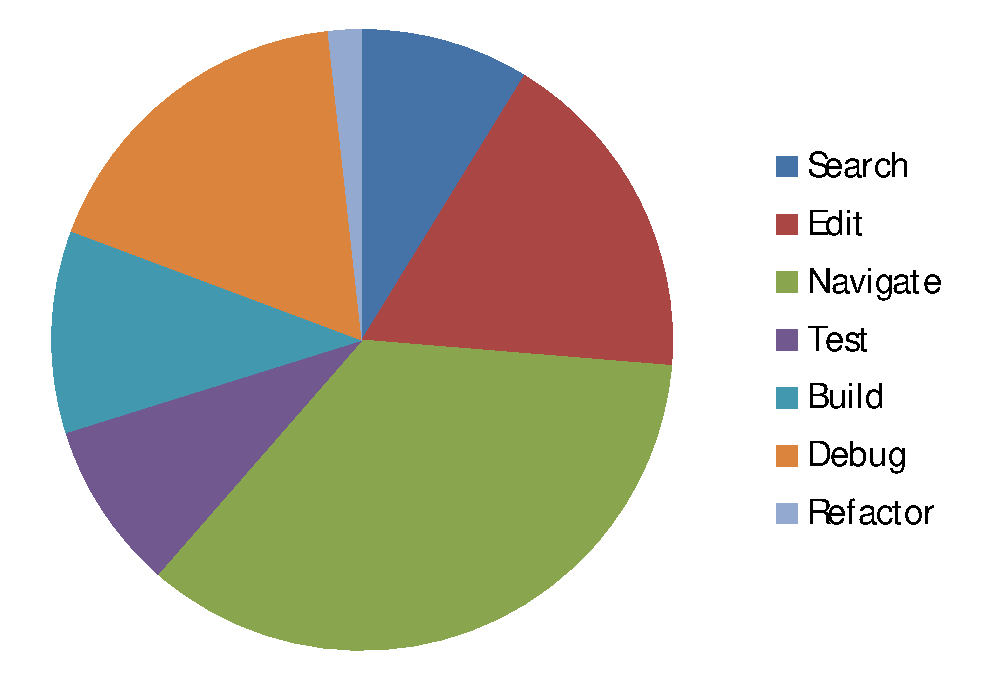
\includegraphics[width=0.5\columnwidth]{../Graphics/activityCategorization.pdf}
%\caption{Pairwise matches across categories, including matching and mismatching pairs.}
%\label{fig:category}
%\end{figure*}


\subsection{Sequence Analysis}
%intro to seqence analysis, sessions
Magnitude analysis and categorization are both appropriate for answering simple research questions. However, a more powerful way of analyzing activity logs is through sequence analysis, which first breaks activity sequences into session, according to some criteria, and then reports upon characteristics of that session. A session is a particular interaction with an IDE by a specific user in order to complete a task (e.g. refactoring, looking for a starting point for a maintenance task, etc.), consisting of all of IDE events in a given time span.
For instance, answering the research question of ``Are developers successful at finding initial points in the code for a software maintenance task?'' requires that the sequence of IDE events corresponding to each maintenance task be identified, before we can perform further analysis using either magnitude or categorization analysis. The granularity of a session is determined by the guiding research question. For certain research questions, we may be interested in a smaller session (e.g. searching the code base), while for others we may need to consider a longer time span (e.g. performing a maintenance task, developing a new feature). 

%how difficult or easy is it to determine sessions
In many cases, extracting sessions from activity sequences can be challenging as it impossible to know exactly when a developer begins or ends a particular task, without understanding his or her underlying thought process. There are several possibilities in how session extraction can be performed, based on the task related to the specific research question. One possibility is to use sentinels, which are specific actions where we can detect a task begins or ends. For instance, in code search, submitting a query to the code searcht tool begin one task and end the prior task in the activity stream. Another possibility is to use the passage of time to extract sessions, where time without any activity is used as a signal of task start or finish. Coman et al.'s \cite{Coman-TaskIdent} algorithm uses a combination of key events in the activity stream and time distance between such events to extract relevant sessions corresponding to developer tasks. In lab validation studies this algorithm has shown very high accuracy (80\%) when compared to the ground truth reported by developers, however this accuracy may not hold up in an industrial setting\cite{Zou-ComanIndustry}.


%example
As an example of sequnce analysis, consider a researcher investigating finding initial points in the code for a software maintenance task. Specifically, the developer is interested in the following research question ``Are users satisfied with file search results?''. This question, while impossible to answer via simple magnitude analysis can be investigated via session analysis. Using assumptions from in-lab studies that show that opening a search result followed by a long pause correlates with user satisfaction we can analyze activitiy logs to determine how often user behavior indicated satisfaction in the field. The researcher may break activity logs into sessions, starting with a search being executed and ending on the last interaction with that result set. He could calculate additional characteristics from this raw data, such as the amount of time spent per session, the number of results reviewed, and the number of files opened.   


\begin{figure*}[t]
 \centering
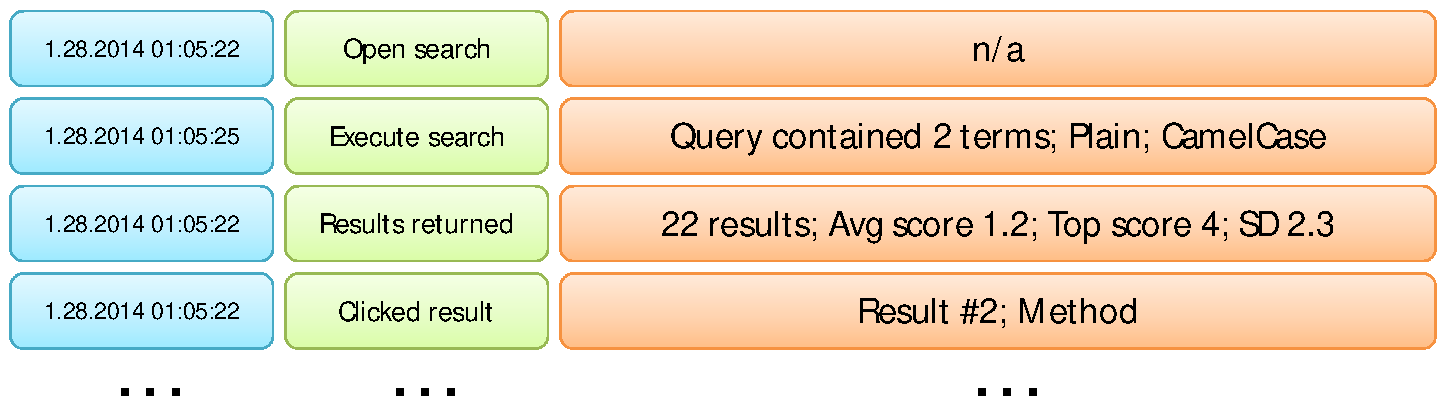
\includegraphics[width=1\columnwidth]{../Graphics/activityLogActual.pdf}
%\caption{Pairwise matches across categories, including matching and mismatching pairs.}
\label{fig:actual}
\end{figure*}

%Sequence analysis is currently the most powerful tool we have for analyzing logs. While there has been preliminary work to complete annotate activity logs into tasks or even states (e.g., editing, searching, navigating, testing, etc.) these analyses are currently unreliable. In fact, we believe that because user behavior is often multi-purposed there will remain major obstacles to inferring higher-level user states from activity streams, ultimately limiting the usefulness of any full log analysis. 




\subsection{State Model Analysis}
Another way to analyze log data is to view the log as a sequence of events occurring in a state machine.  Using state models, we can quantify the occurrences of repeating actions and describe a usage pattern in statistical analysis.  In state model analysis, the sequential data is converted to nodes and edges of a graph which represents the entire data in states and transitions between them.  A Markov state model provides information about the probability of occurrence of each state and the transitional probability of each activity.   The statistics provided in a Markov state model include the quantity of time and probability for the developer being in each state.  From a given state, the model calculates the probability of each transition to different unique states.  State models answer specific questions such as what is the probability that once a developer searches the code, they edit a code element listed in the find results. Expanding this question, the probability of an entire use case or set of transitions through the usage model, is calculable from the state model.  

State model graphs make it easy to identify the most active states and edges provides information about the important activities in the data set.  As the number of states increases, the WDG becomes more complex and hence difficult to understand.  When this occurs, summarizing the detailed event data into higher-level categories effectively combines the states to get more meaningful information.   For example, classifying events in usage data of similar types into categories results in fewer states with the same number of transitions as the original data.

We generate a state model from a usage log by transforming the serially ordered events in a sequence data to a Weighted Directed Graph (WDG) data structure.  We can abstract the information in the log line to any level, such as, event level, event category level, tool level, or application level. In the sequence data, each event is important as a standalone event, however, in the WDG representation, the importance shifts to adjacent pairs of events. 
%We do this type of a transformation to record the order in which events happened. 
Therefore, each unique event in the sequence data is represented by a unique node in the WDG. 

To understand how to interpret a state model, look at our example graph figure \ref{op-profile-example}.  We see that an edge exists from one node (head) to another (tail) if there is an occurrence of the event representing the tail node immediately after the event representing the head node in the  log file. For example if event B follows event A in the log file, then there is directed edge from node A to node B in the WDG. The edges are labeled with the number of times this transition has occurred.  For example if B occurs a fifty times after A in the log file, then the edge from node A to node B in the WDG is labeled with 50. Typically, we keep track of the actual count as the weight of the edge, when building the graph. In the graph we display the percentage value as the label. This percentage is proportional to the total number of transitions.  The cumulative probability of out-edges of a node is 1. The transitional probabilities of each out-edge is calculated by dividing the number of transactions of that out-edge with the sum of all outward transactions from that node. We could also store the dynamic parameter information in each log line as a list along the edges. 

As an example, consider a sample log file shown in figure \ref{samplelogfile} given below and the corresponding state model graph in figure \ref{op-profile-example}. Intuitively you can see how the state model represents the log states and transitions between them in the sequence of events.  

\begin{figure}
\hrulefill
\begin{verbatim}
2013-03-21 18:18:32Z,A
2013-03-21 18:18:33Z,B
2013-03-21 18:20:49Z,C
2013-03-21 18:20:50Z,A
2013-03-21 18:20:56Z,B
2013-03-21 18:20:57Z,A
2013-03-21 18:21:08Z,C
2013-03-21 18:21:08Z,D
2013-03-21 18:21:08Z,E
2013-03-21 18:21:08Z,A
\end{verbatim}
\hrulefill
\caption{Sample Log File to Convert to State Model}\label{samplelogfile}
\end{figure}

\begin{figure}[h]
  \centering
  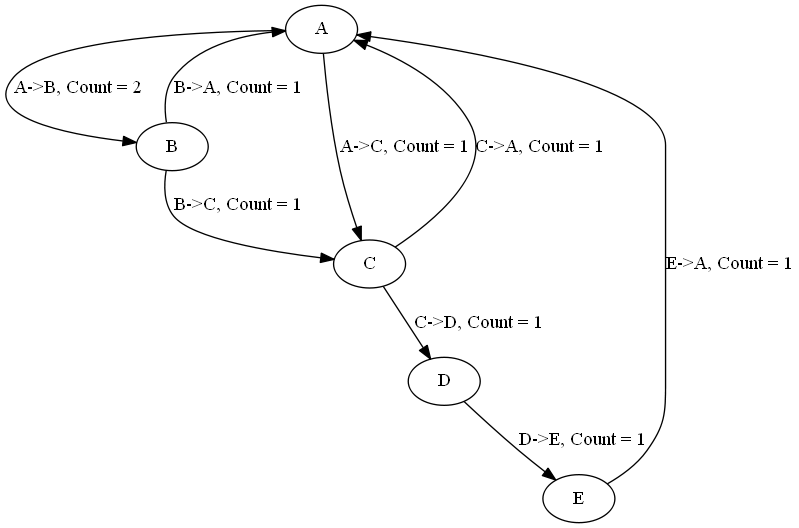
\includegraphics[scale=.40]{op-profile-example.png}
  \caption{Weighted Directed Graph of the Example Log}\label{op-profile-example}
\end{figure}






%the other example is aligned with the sample graph thus better.
%As an example of WDG, consider a simple log file where the activities are separated by commas. $1-2, 2-3, 3-4, 4-5, 5-4, 4-5, 5-4, 4-6, 6-7, 7-5, 5-4, 4-5, 5-4, 4-5, 5-8, 8-9$. The events in the log file are mapped to their corresponding event IDs: $1, 2, 3, 4, 5, 4, 5, 4, 6, 7, 5, 4, 5, 4, 5, 8, 9$. Each node is a unique event. An edge between nodes 1 and 2 signifies that the event 2  appears after event 1  in the log file. The labels on the edges have the actual count and could have the transitional probabilities as well. The transitional probability from node 1 to node 2 is 1.0, whereas the transitional probability from node 4 to node 6 is 0.2.  This is depicted in Fig \ref{op-profile-example}.
 
Converting a log into a state model requires three steps.  We use JUMBL (Java Usage Model Builder) from the Software Quality Reasearch Laboratory (SQRL) of the University of Tennessee.    Details on input formats and JUMBL tools are available on sourceforge at \footnote{\url{http://jumbl.sourceforge.net/}}.
\begin{enumerate}
\item
First, convert the log file into a representation for each transition called a sequence based specification. The format for a sequence based specficicaiton in csv files is described in the JUMBL user guide. This representation contains the following information with one row for each transition :
\begin{itemize}
\item State transition
\item Count of transitions
\item Total time elapsed
\item State In information
\item State Out information
\end{itemize}

\item
After importing the sequence based spec, JUMBL can write out the representation of a state model as a TML script or several other formats including GML (Graph Modeling Language) that graph tools can import.  The TML  has information about the nodes, the out edges from each node along with the number of transitions from each node to another. The corresponding graph for the usage log example is depicted in Fig. \ref{op-profile-example}
\end{enumerate}


Using state models, a sequence data with hundreds of thousands of lines can be quickly converted to more meaningful graphical representation using this method. Once the TML file is generated, we can use JUMBL to find out the state probabilities of each states. Using the state probability and the usage patterns we can draw conclusions about the occupancy of individual states and the use cases that involve transitions through several states.

%Trying this on without the following examples.  They don't really add much and raise more questions than they answer.  I hope reference take care of the how to in this case.


%
%\begin{figure}
%\label{sampleTML}
%\hrulefill
%\begin{verbatim}
%($ fill(1) $)
%model testlog
%//use this before each transition to show probability ($0.10$)
%
%source [A]
%($2$)"Count=2 (A->B), TimeElapsed= 7secs" [B]
%($1$)"Count=1 (A->C), TimeElapsed= 11secs" [C]
%
%[B]
%($1$)"Count=1 (B->C), TimeElapsed= 136secs" [C]
%($1$)"Count=1 (B->A), TimeElapsed= 1secs" [A]
%
%[C]
%($1$)"Count=1 (C->A), TimeElapsed= 1secs" [A]
%($1$)"Count=1 (C->D)" [D]
%
%[D]
%($1$)"Count=1 (D->E)" [E]
%
%[E]
%($1$)"Count=1 (E->A)" [A]
%
%
%"exit" [Exit]
%
%end 
%\end{verbatim}
%\hrulefill
%\caption{Sample TML for a State Model}
%\end{figure}



%%I commented these out because they were out in space in the document and not well supported by the text.  You probably cut the text because of other comments.  Anyhow does it make sense to stick with one WDG example based on the state model shown in text above?  Seems OK to me so far. 

%\begin{figure}
%  \centering
%  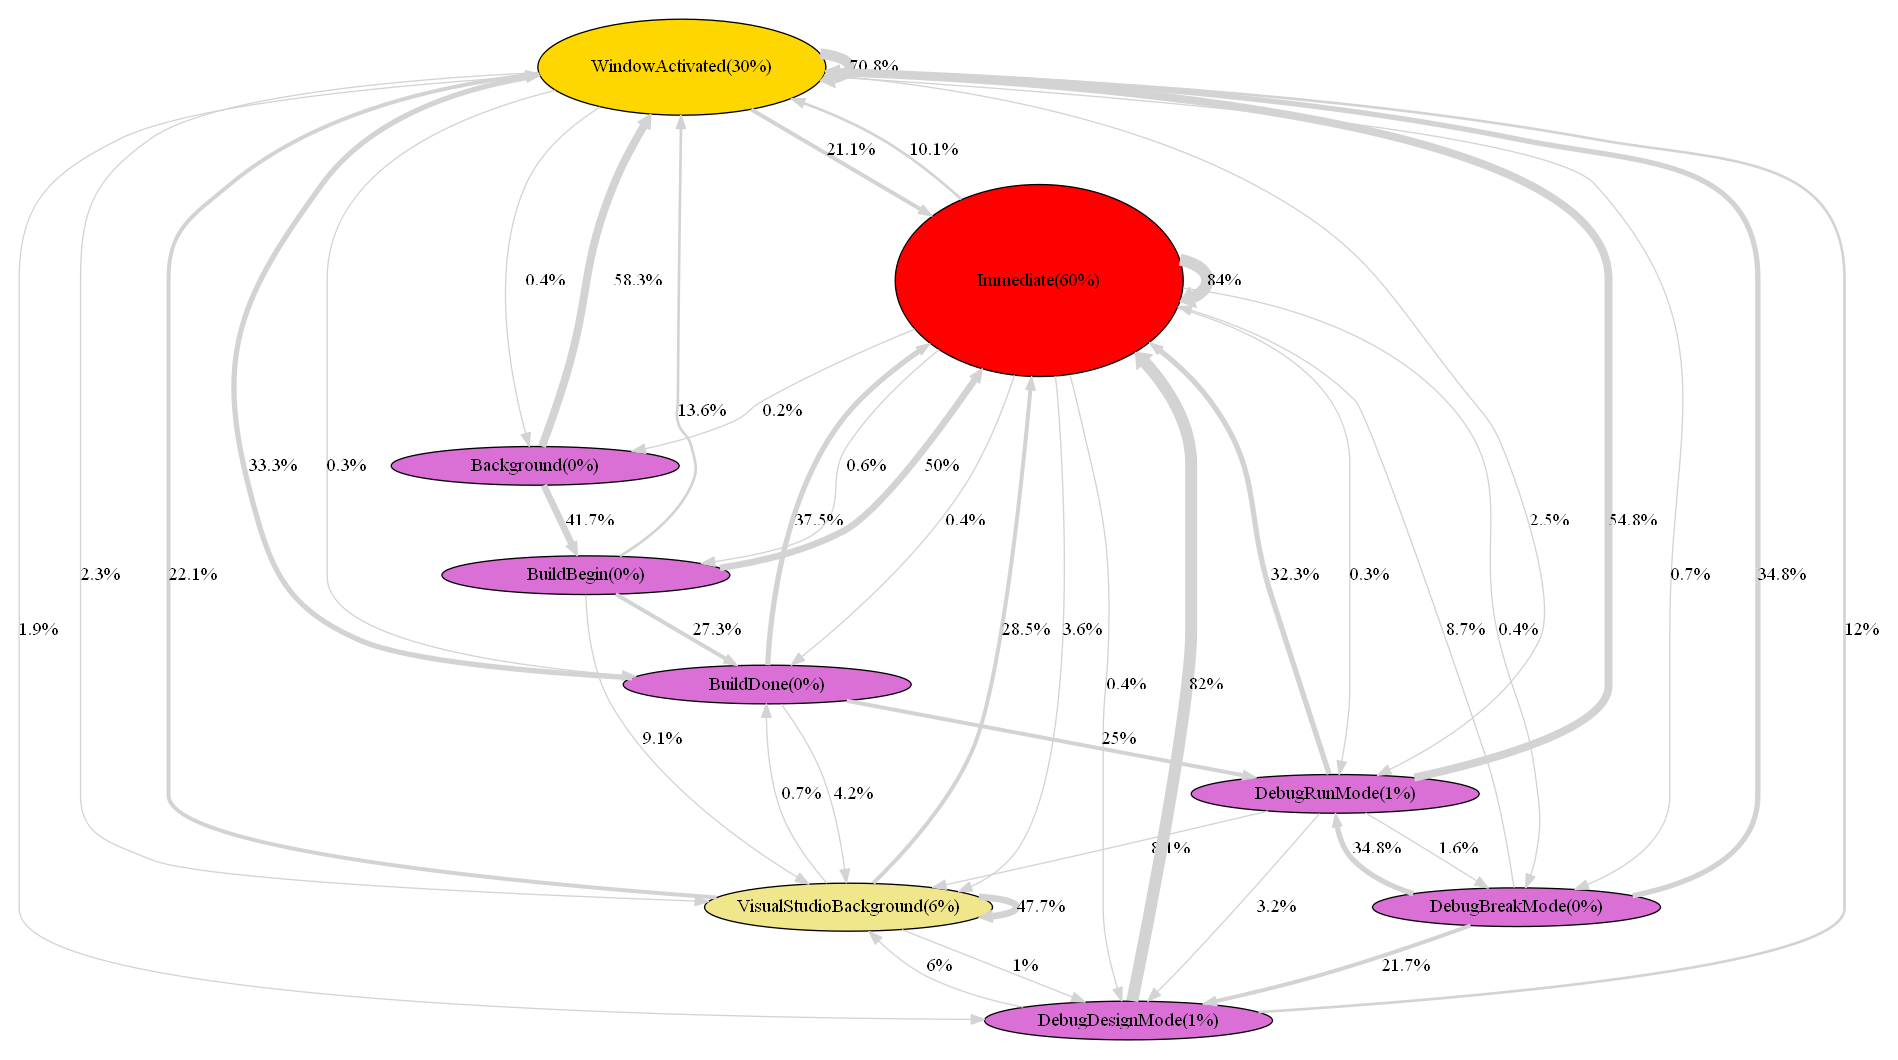
\includegraphics[scale=.15]{log_with_color.png}
%  \caption{WDG example with probability}\label{fig:log_with_color}
%\end{figure}

%\begin{figure}
%  \centering
%  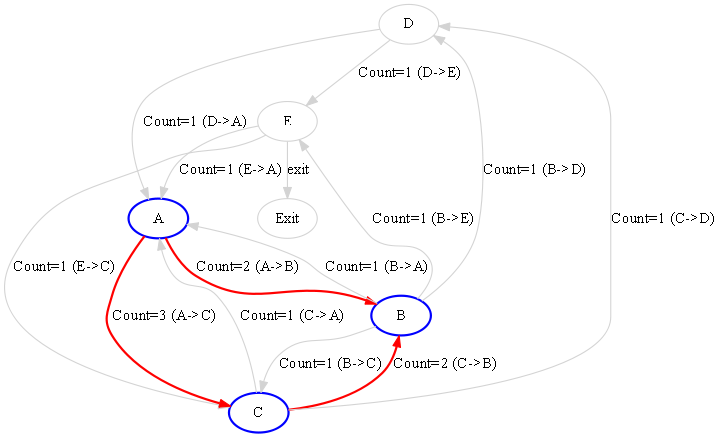
\includegraphics[scale=.50]{sample_log.png}
%  \caption{WDG example with count}\label{fig:sample_log}
%\end{figure}

 




\subsection{Research combining usage data with other sources}


Other data sources, such as task descriptions, change histories, and
news feeds can provide context for usage data and yield new opportunities for supporting developers. In this section, we briefly outline some related work in this area.
% that combines usage data with other data sources to a new set of applications. In this section, we outline the related work that combines usage data with other software engineering data sources.

\subsubsection{Tasks}

%Mylin
As mentioned above, Mylin is a popular extension to the Eclipse IDE that supports task
management, reducing the effort for a developer to switch between
tasks and maintaining relevant information for each
task~\cite{Kersten-Mylin}. In the context of a specific task, Mylin
collects usage data in order to compute a degree-of-interest (DOI)
value for each program element, which represents the interest the
developer has in the program element for the task at hand. Program elements that a developer interacted with frequently and recently have a higher DOI value. Using these calculated DOI values, Mylyn highlights the elements relevant for the current task and filters unnecessary information from common views in the IDE. 

\subsubsection{Change History}

%FastDash
The FastDash tool enables real-time awareness of other developers'
actions (e.g. focus or edits to a specific file) by utilizing usage
data in concert with the source files and
directories~\cite{FastDash}. FastDash's purpose is to reduce faults
caused by lack of communication and lack of awareness of activities
that other developers are performing on the same code base. The tool
highlights other developer's activity as it is occurring using a
sophisticated dashboard on the developer's screen or on a team's dashboard.

